%=================AVANCES Y PRUEBAS=================
% SENSORES DE PULSO

\section{Sensores de pulso}
La prueba se realizó para visualizar la onda de salida entregada por ambos sensores en un osciloscopio y verificar su funcionamiento. 

\subsection{AD8232}

El primer sensor que fue probado es el AD8232, el cual es de tipo ECG y utiliza tres electrodos que se deben colocar en el brazo izquierdo y derecho, y la pierna derecha. 

El sensor fue alimentado con 3.3 V.

En las siguientes imágenes se muestran las conexiones realizadas y la onda entregada en el osciloscopio.
	
\subsection{Pulse sensor}	

	\begin{figure}[htbp!]
		\centering
		\fbox{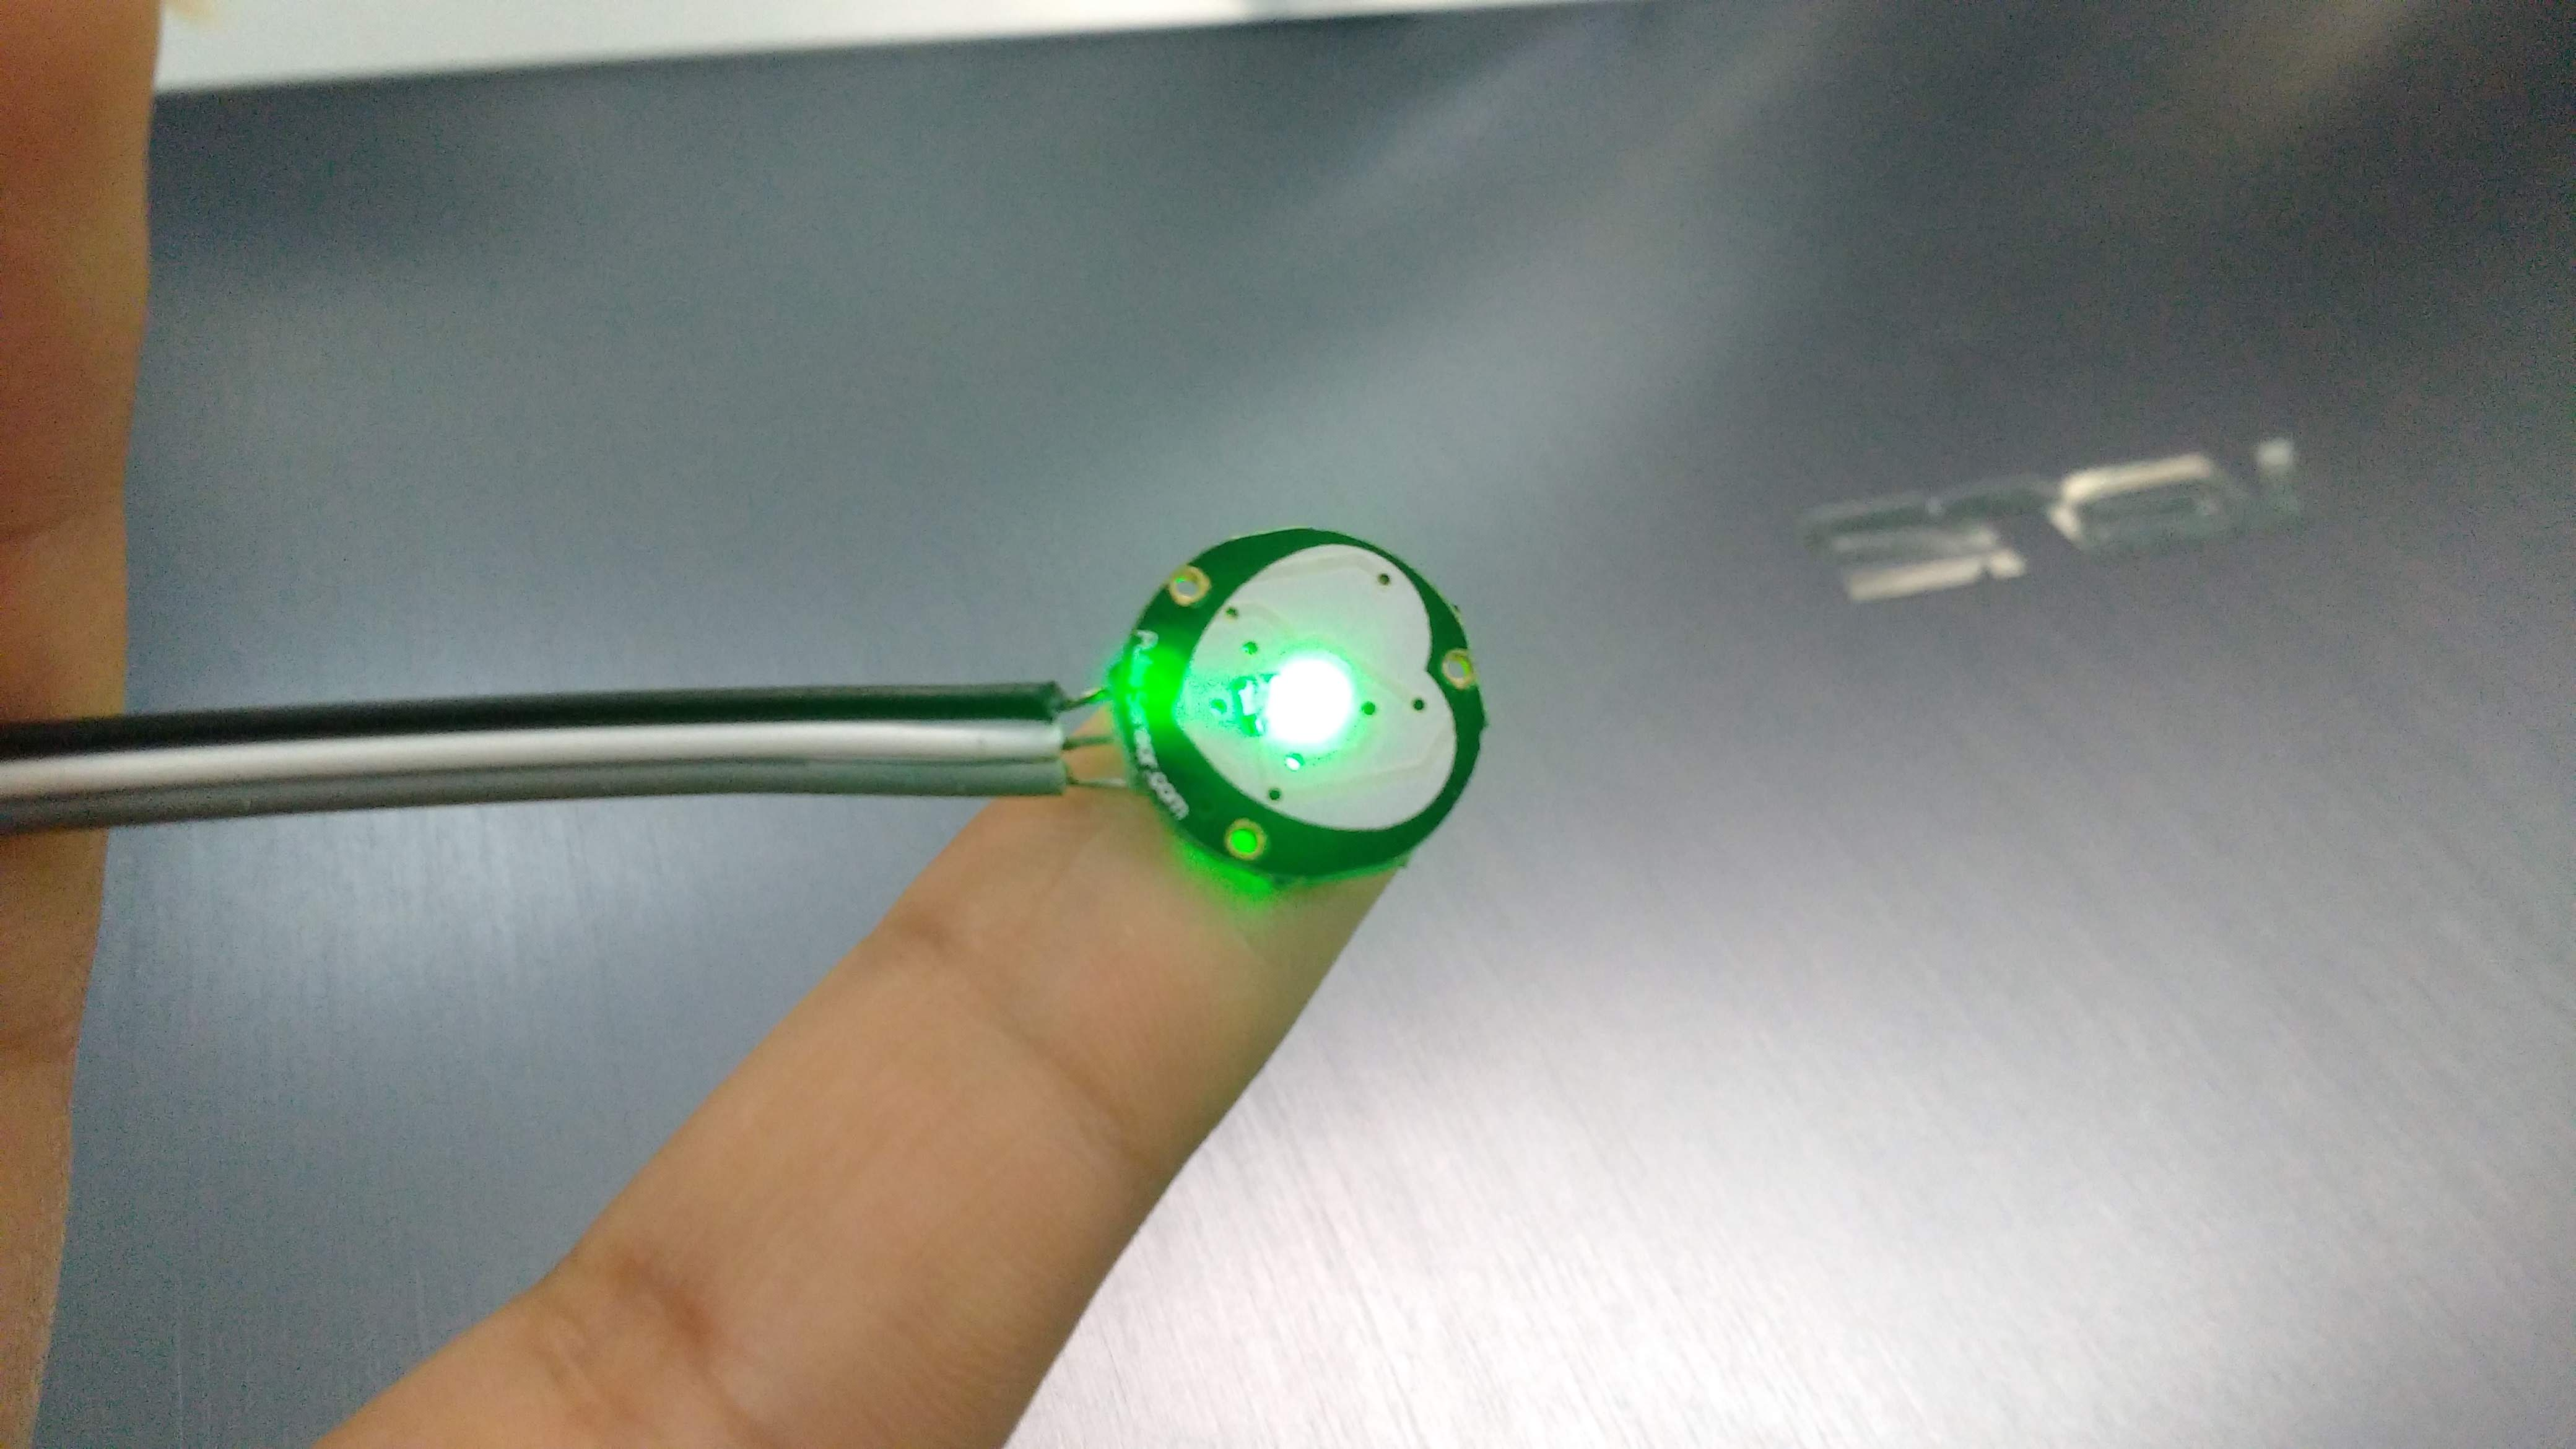
\includegraphics[width=0.6\textwidth]{AvancesPruebas/imagenes/PulseSensor2.jpg}}
		\caption{Prueba del sensor de pulso.}
		\label{fig:PulseSensor2}
	\end{figure}
	
	\begin{figure}[htbp!]
		\centering
		\fbox{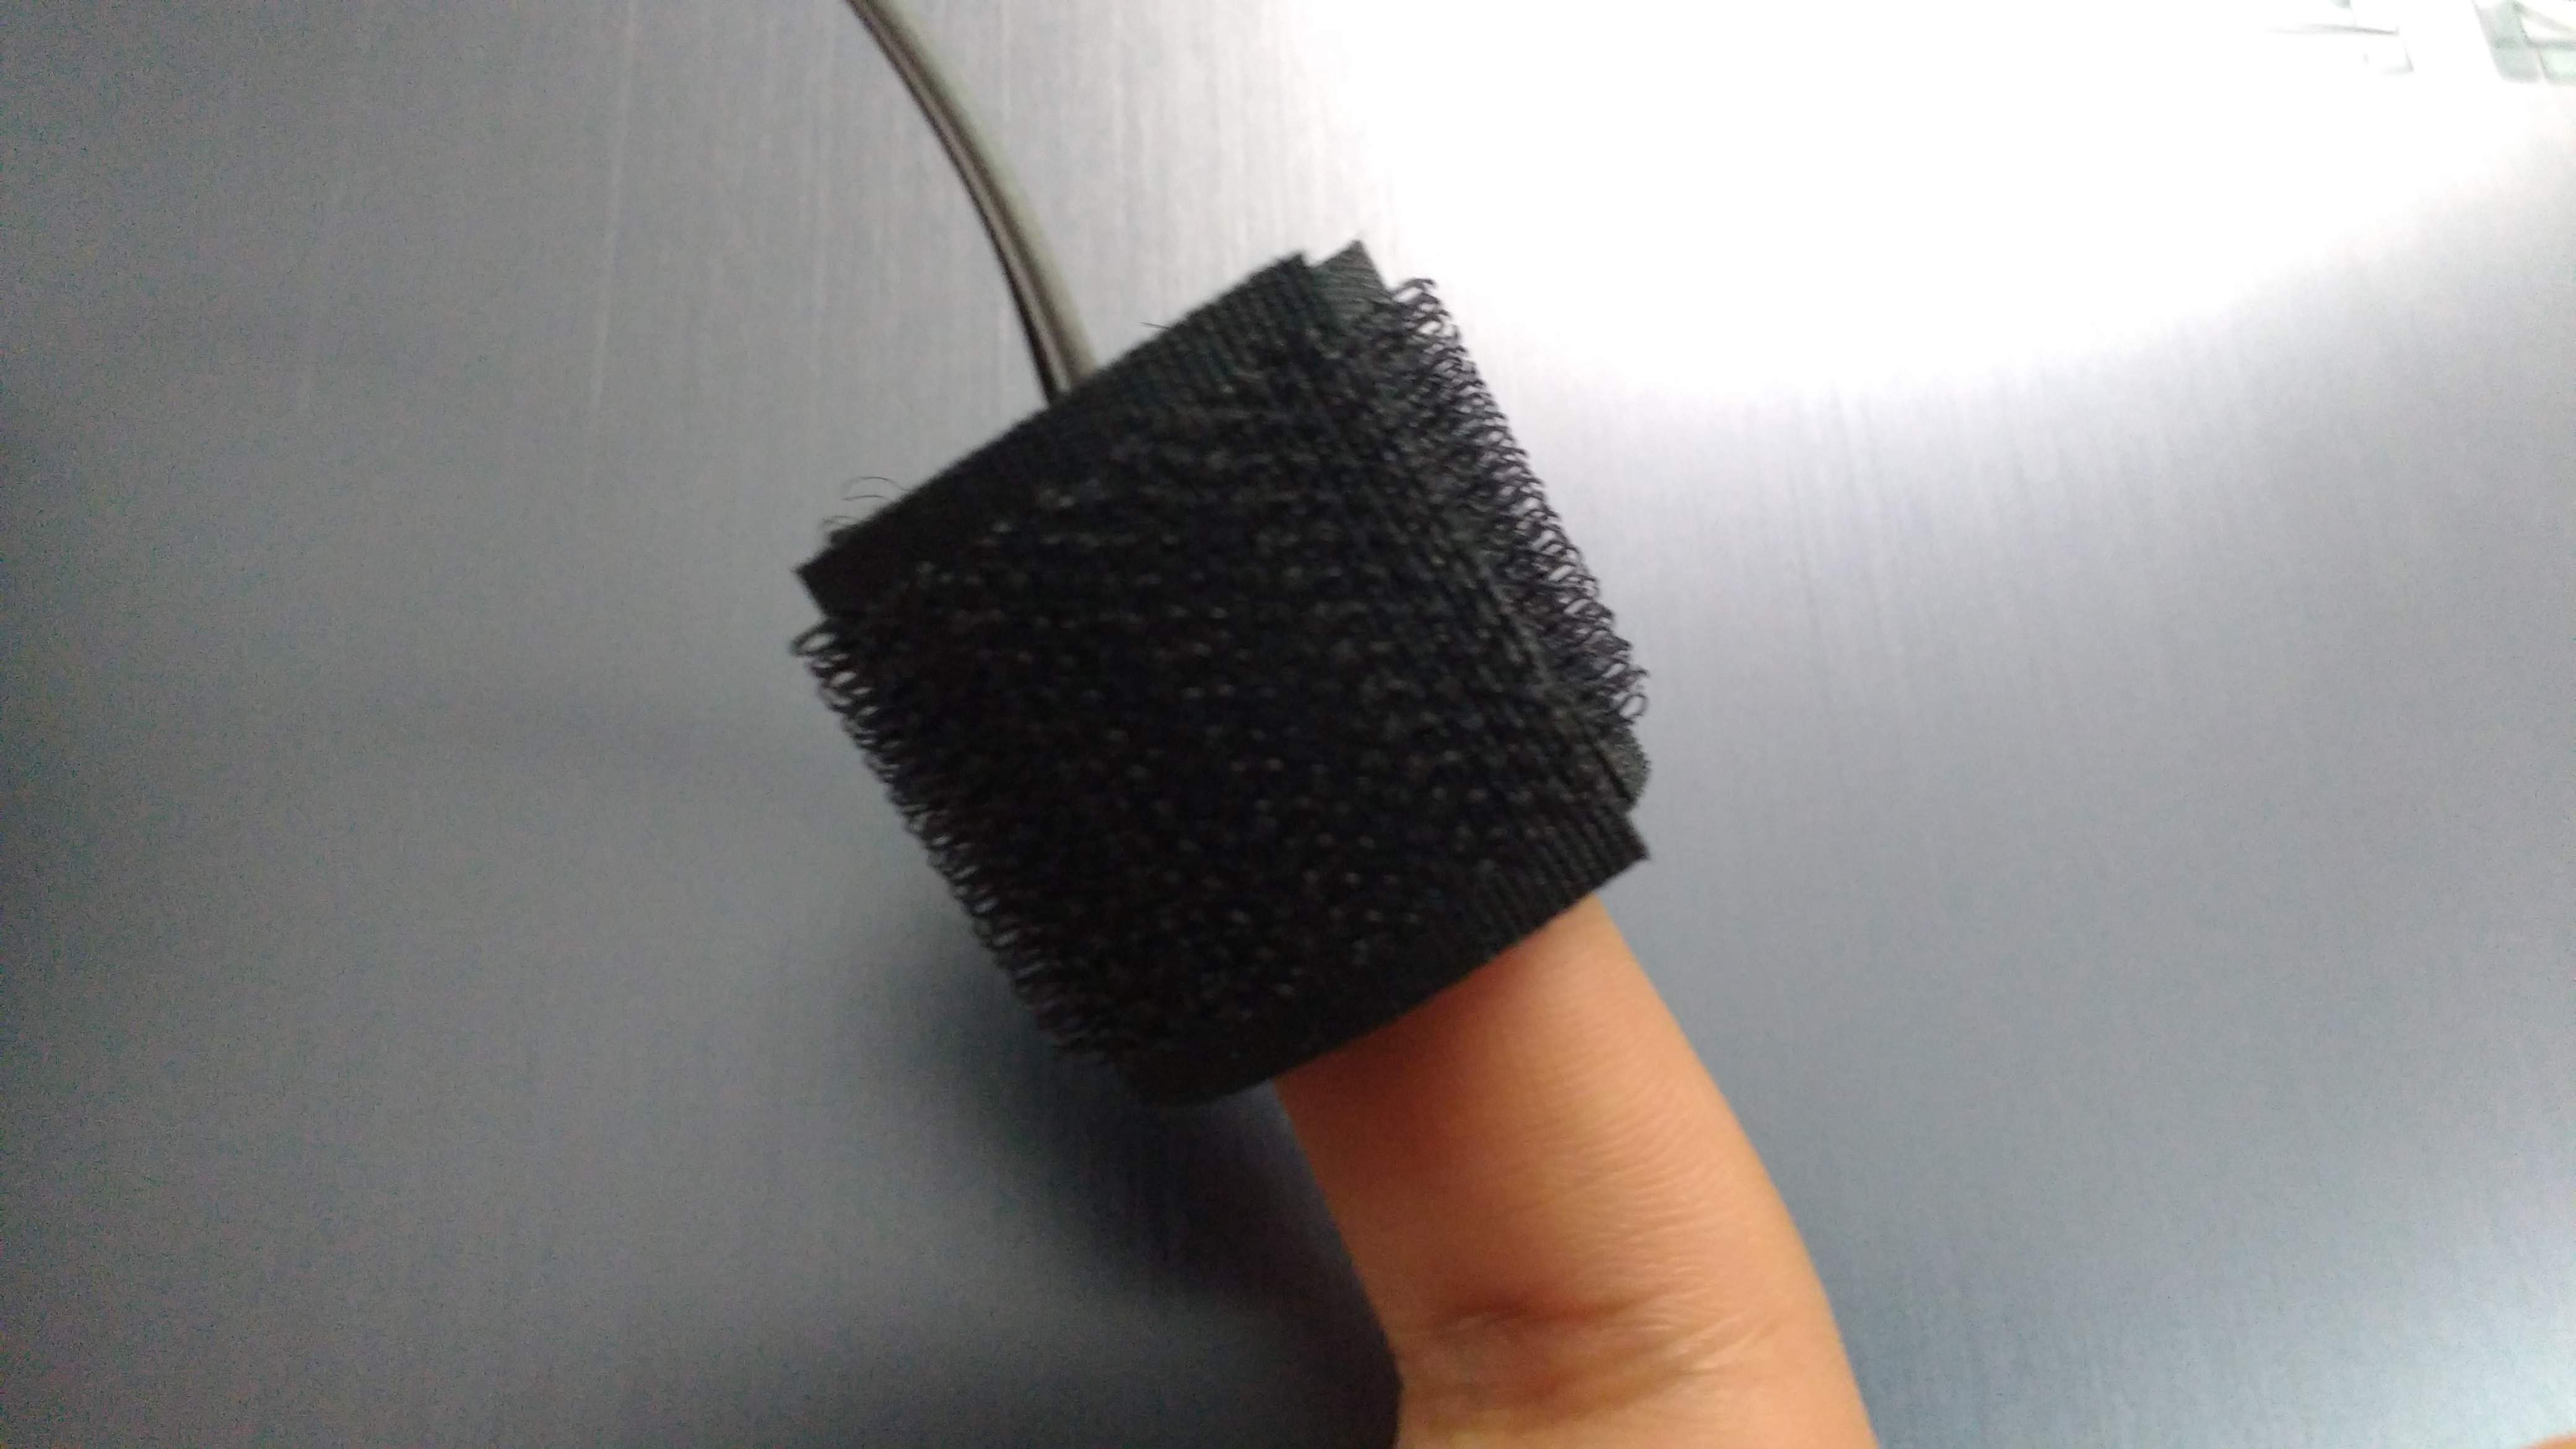
\includegraphics[width=0.6\textwidth]{AvancesPruebas/imagenes/PulseSensor1.jpg}}
		\caption{Prueba del sensor de pulso.}
		\label{fig:PulseSensor1}
	\end{figure}
	
	\begin{figure}[htbp!]
		\centering
		\fbox{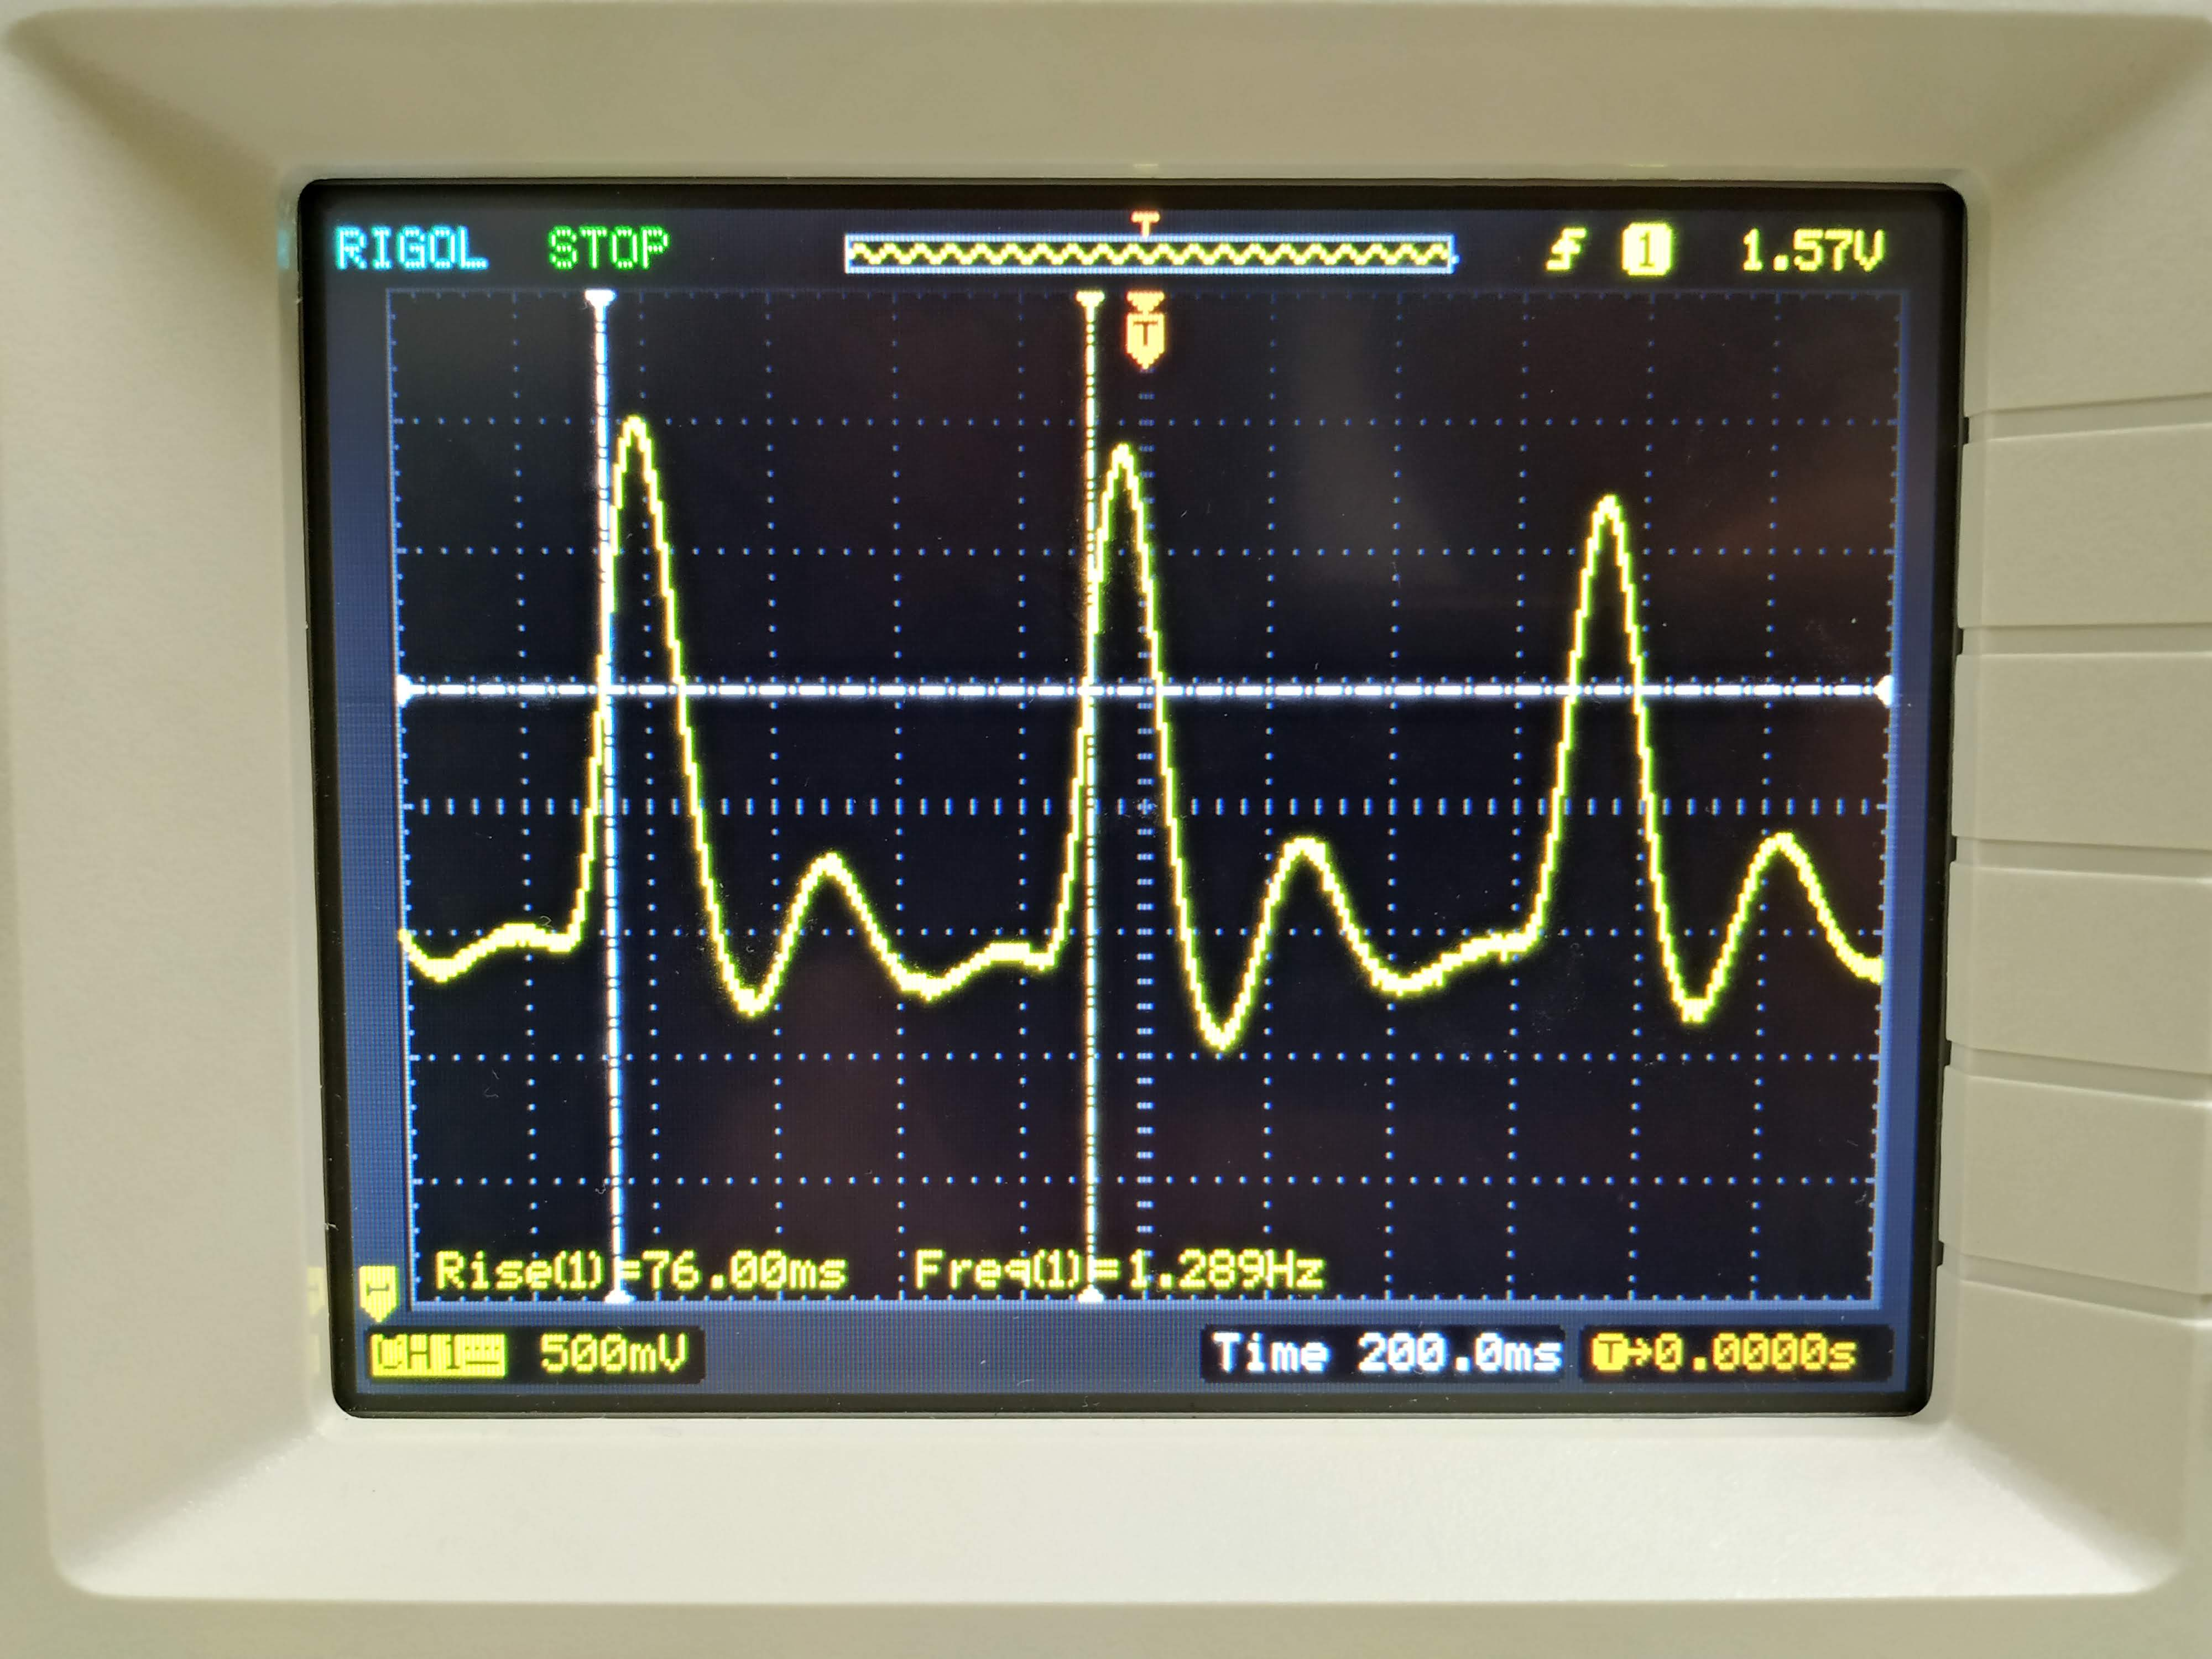
\includegraphics[width=0.6\textwidth]{AvancesPruebas/imagenes/PulseSensor3.jpg}}
		\caption{Prueba del sensor de pulso.}
		\label{fig:PulseSensor3}
	\end{figure}
	
\section{Digitalización de señal analógica}


	\begin{figure}[htbp!]
		\centering
		\fbox{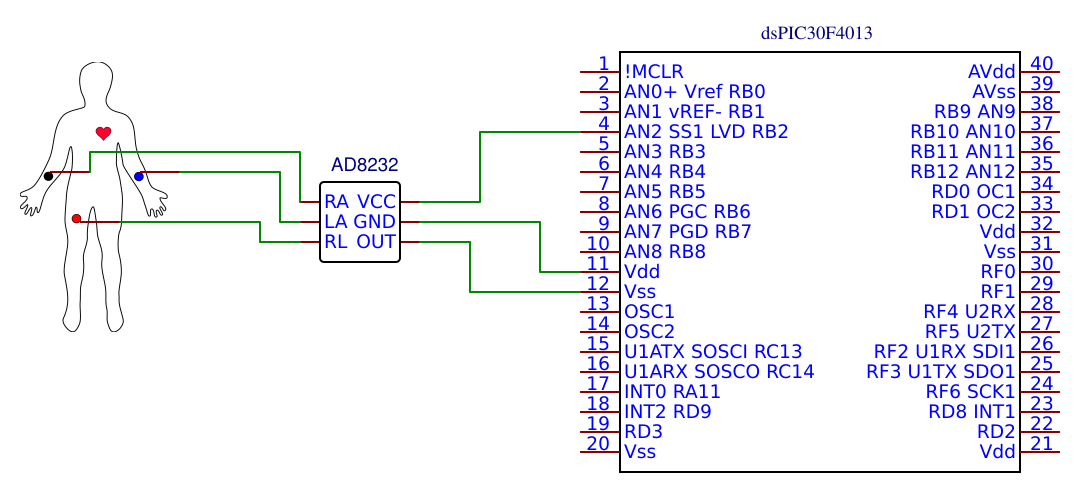
\includegraphics[width=\textwidth]{AvancesPruebas/imagenes/AD8232Conexion.png}}
		\caption{Conexión de AD8232 con dsPIC30F4013.}
		\label{fig:ConexionAD8232}
	\end{figure}
	
	\begin{figure}[htbp!]
		\centering
		\fbox{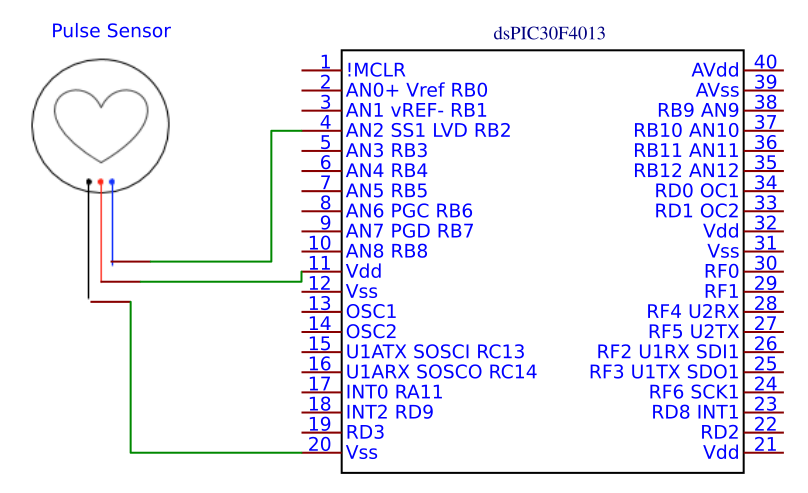
\includegraphics[width=0.8\textwidth]{AvancesPruebas/imagenes/PulseSensorConexion.png}}
		\caption{Conexión de PulseSensor con dsPIC30F4013.}
		\label{fig:ConexionPulseSensor}
	\end{figure}
	\pagebreak
	
\section{Conexión del módulo Telit GL865-QUAD}
Para verificar que el módulo tenga un correcto funcionamiento, se probó de manera unitaria el UART del módulo Telit GL865-QUAD con un módulo FT232. La conexión entra ambos componentes se realizó de forma cruzada, es decir, que el transmisor de un dispositivo fue conectado al receptor del otro , tal como se muestra en la figura \ref{fig:ConexionUART}.

	\begin{figure}[htbp!]
		\centering
		\fbox{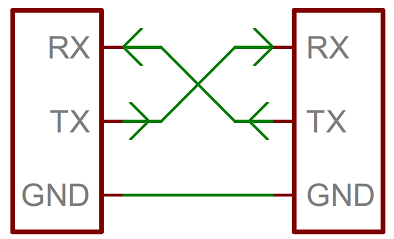
\includegraphics[width=0.4\textwidth]{AvancesPruebas/imagenes/conexion-uart.png}}
		\caption{Conexión UART de módulo GSM y FT232}
		\label{fig:ConexionUART}
	\end{figure}
	
Una vez conectado correctamente ambos módulos, se realizó la prueba de la siguiente forma:
\begin{enumerate}
	\item Se ejecutó el emulador de terminal ’PuTTY’, configurándolo para el puerto serial
	indicado, con un baudaje de 9600, transmisión de 8 bits, sin paridad con 1 bit de
	stop y sin flujo de control. La configuración realizada se muestra en la figura \ref{fig:ConfiguracionPutty}.
	\item Se ejecutaron los comandos AT básicos para probar el módulo GL865-QUAD, en ninguno de ellos
	debe aparecer un error, de lo contrario se debe revisar la conexión entre los dispositivos
	y la instalación del software necesario. Algunos de los comandos utilizados, son:
		\begin{enumerate}
			\item AT
			\item AT+GSV
			\item AT+IPR=?
			\item AT+CSQ
			\item AT+CREG? 
			\item AT+CGREG? 
			\item AT+CGNSPWR=1
			\item AT+CGNSINF=0
		\end{enumerate}	
\end{enumerate}
 
	\begin{figure}[htbp!]
		\centering
		\fbox{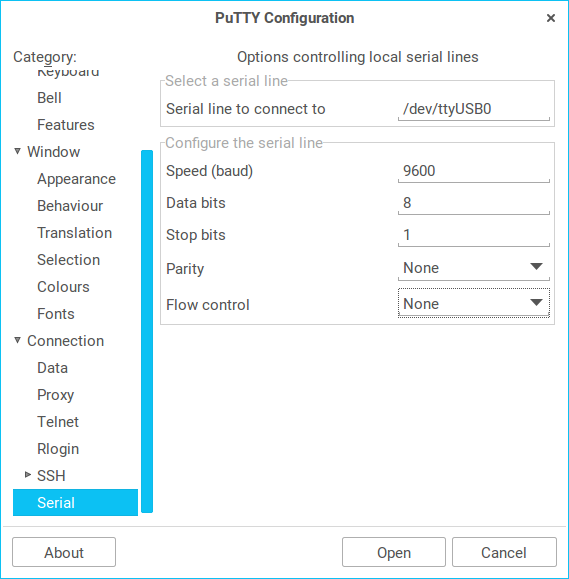
\includegraphics[width=0.5\textwidth]{AvancesPruebas/imagenes/putty.png}}
		\caption{Configuración de terminal en PuTTY}
		\label{fig:ConfiguracionPutty}
	\end{figure}
 
El resultado de los comandos ejecutados mediante la terminal de PuTTY se muestran en la figura X.